\chapter{System architecture}
\label{chap:systemarchitektur}

Building on the requirements of the system described in chapter \ref{chap:systemanforderungen}, this chapter will present a draft of the system architecture. Since CouchApp applications allow an architecture with no middleware, the focus lies less on the presentation of the components. Rather, the inner structure of the application will be described. The concepts for the central design problems will be discussed and every choice will be accounted for. This will convey an overview of data storage functionality, application logic and the user interface.

The code snippets in this chapter are no complete CouchDB documents. They only contain what is strictly necessary for the demonstration of certain aspects.

\section{Architecture overview}

Conventional web applications are built according to \textit{client-server} architecture: the data reside in a usually relational database, the application logic is executed on the server and the results are sent to the client (see fig. \ref{fig:old-web-arch}). Only some parts of the application logic are sometimes executed by the browser as an add-on to enhance user experience.

\medskip
\begin{figure}[ht] 
  \begin{center}
    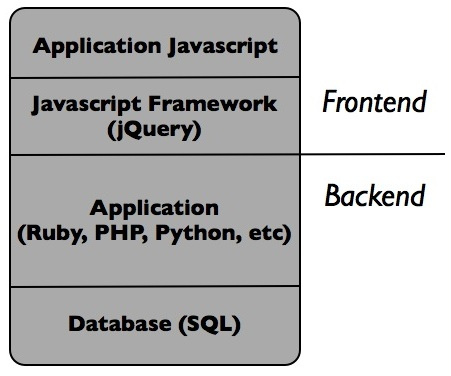
\includegraphics[width=0.5\textwidth]{grafik/old-application-architecture} 
  \end{center}
\caption{Architecture of a conventional web application, according to \cite{web:architecture}}
\label{fig:old-web-arch} 
\end{figure}

If one assumes that the browser supports JavaScript and HTML5, larger parts of the application can be run locally on the user's computer. CouchDB furthermore provides its own web server. This eliminates the need to use middleware for the application logic (see fig. \ref{fig:new-web-arch}).

\medskip
\begin{figure}[ht] 
  \begin{center}
    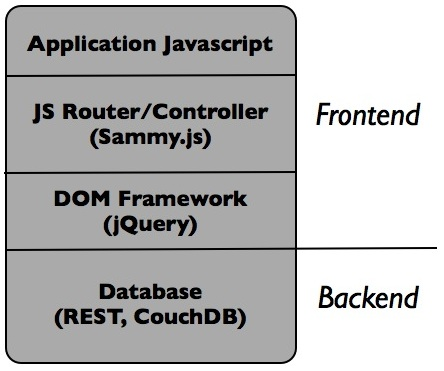
\includegraphics[width=0.5\textwidth]{grafik/new-application-architecture} 
  \end{center}
\caption{Architecture of a CouchApp, according to \cite{web:architecture}}
\label{fig:new-web-arch} 
\end{figure}

\afterpage{\clearpage}

If CouchDB is installed onto a local computer, the application may be run like a desktop program. The server instance's only responsibility is the synchronisation of outlines between clients (see fig. \ref{fig:projektvision}). It is sufficient to implement a single application that runs on the clients as well as the server. The application can also be used on the clients when the server is unavailable.

\medskip
\begin{figure}[H] 
  \begin{center}
    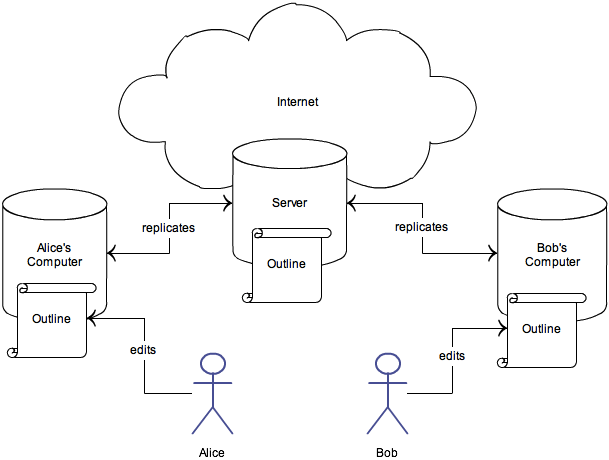
\includegraphics[width=0.85\textwidth]{grafik/Projektvision} 
  \end{center}
  \caption{Project vision}
  \label{fig:projektvision} 
\end{figure}


\section{Data structure modelling}

For the storage of data in the database, there were several alternatives. The discussion of these will justify the solution chosen.

\subsection{Requirements}
\label{subsec:ana-anf}

The requirements for data structure modelling are prioritised as follows:

\begin{itemize}
  \item It should be easy to program and maintain the application.
  \item Conflicts caused by simultaneous saving of data should be avoided or occur as infrequently as possible.
  \item Data access should be as fast as possible. Since less requests reduce access times, related data should be stored together wherever possible.
\end{itemize}

CouchDB's replication can automatically highlight conflicting documents. A workable application, however, will require some logic that allows these conflicts to be resolved. The data structure was designed with advice taken from \cite{design:replication}.

\subsection{Problem}

An outline is a sorted, hierarchically nested list of lines with varying indentation. A simple example is illustrated in figure \ref{fig:nestedoutline}. The bullets for lines that have no child nodes are circles, and triangles for lines that do. Such an outline should be implemented meeting the requirements mentioned above.

In the example a shopping list is composed with the aid of the outliner. This is indeed not the main purpose of an outliner, but it illustrates the hierarchical indentation in an intuitive way, and it allows the example to remain short yet realistic.
 
\medskip
\begin{figure}[ht] 
  \begin{center}
    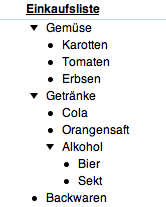
\includegraphics[width=0.3\textwidth]{grafik/nested-outline} 
  \end{center}
  \caption{Simple outline}
  \label{fig:nestedoutline}
\end{figure}

\subsection{Storage in a JSON document}

The easiest implementation is saving everything into a single JSON document (see listing \ref{lst:nestedoutline}). For this approach, every line has to be a JSON object in itself, so that they can be stored in their nested state.

This outline will temporarily exist in two or more different versions during the application's lifetime. On the next synchronisation of both versions they should again be merged. Lines that were altered, added or deleted should also be altered, added or deleted in the other version. The user should only have to intervene when a line has two competing versions. How can this be achieved?

\medskip
\begin{lstlisting}[caption=Simple outline in a JSON document, label={lst:nestedoutline}]
{
  "title": "Shopping list",
  "lines": [
    {"text": "Vegetables", "lines": [
      {"text": "Carrots"},
      {"text": "Tomatoes"}, 
      {"text": "Peas"}
    ]}, 
    {"text": "Drinks", "lines": [
      {"text": "Cola"},
      {"text": "OJ"}, 
      {"text": "Alcohol", "lines": [
        {"text": "Beer"},
        {"text": "Champagne"}
      ]},
    ]},
    {"text": "Pastries"}
  ]
}
\end{lstlisting}


The structure in listing \ref{lst:nestedoutline} is already valid JSON. It could be stored as-is in a single CouchDB document. This document could be read with a single read operation. The replication of such a document is also done in just one action. Even the implementation of application logic is relatively easy, because the indentation information is contained within the document.

However, problems may arise as soon as the document is modified. When a line is changed, added or moved, CouchDB saves a new version of the outline document with a new revision number. Without exception, conflicts occur every time the outline is replicated with another user's version after the modification took place.

After a replication with many changes in the document, too, there are only two different line sets. One set will be stored as the winning, the other as the conflicting revision. This semantic is very impractical to the user: she can only save either her own or the other version. All changes have to be repeated by hand. This voids some of the central advantages of CouchDB's replication.

\subsection{System prevalence}

Another option is to make use of \textit{system prevalence} \cite{prevalence}. This persistence technique is used in object databases such as Madeleine \cite{madeleine}. Rather than newer versions of the outline, the database records individual operations to the original data set. This way, \enquote{change}, \enquote{save}, and \enquote{move} are single entries in the history of an outline. These entries are stored one after another and never changed. In doing so, no conflicts arise during their replication. The entries can be saved in an array in a single CouchDB document. If replication conflicts occur, they can be easily resolved by combining the elements of both arrays.

However, this approach would also produce problems when different versions are merged, since the order in which changes are made may influence the result. It would be necessary to develop an algorithm that determines the order of the changes in a meaningful way.


\subsection{Version history storage}

Rather than saving the history of the commands, it would be sensible also to save the outlines' older revisions. CouchDB deletes old revisions when the database is compacted. In order to circumvent this, revisions may be saved permanently in their own documents. The system should save a reference to the most recent version and every revision should point to its predecessor. When documents are merged after replication, both conflicting versions may be evaluated until the last common predecessor is found. Based thereon, the merging may proceed.

This is similar to the way versioning systems like Git or Subversion work, except that JSON fields are being compared instead of lines in a text file.

Following this approach, every write operation will also cause the entire outline to be saved as a new version. This means that the database quickly accumulates huge amounts of data. This is a considerable drawback. On merging, both document versions have to be analysed by the application to establish which line was changed in which way and in which version. This process was tested with the aid of a simple prototype with limited functionality, yet quickly rejected for being too complex. Instead, a method should be developed that performs the breakdown already in the document, in order to comply to the quality requirements dictating limited complexity.

\subsection{Breaking up lines in individual JSON documents}

The final approach that was examined involves saving every line in its own document. Adding or deleting a line is achieved by creating or deleting the corresponding JSON document. This method does not necessarily give rise to conflicts. Changing a line will only produce conflicts when both sides change this line at the same time. Only then, user intervention is required. This way, the replication issue is relatively easily solved by the application.

This way of modelling the problem results in many smaller documents in the database, each of which contains only one line. This requires the introduction of an attribute that allows an outlines' lines to be easily recognised in the database. Every line document contains a reference to the outline it belongs to.

This approach brings about the problem that nesting and sorting information is no longer contained inside the document. The solution to this problem will be treated separately in section \ref{sec:sortierung}.

\subsection{Conclusion}
\label{subsec:viewabfrage}

All four solutions have one thing in common: the history of the data has to be saved in some way. Only then it is possible to compare -on merging the replicas- the current state of the data with the state in which the versions did not yet differ. CouchDB saves different versions of documents; it makes sense to make use of this feature. The easiest and least error-prone way is therefore to save lines as individual documents. This is exemplified in listings \ref{lst:outlineforview} and \ref{lst:linesforview}.


\medskip
\begin{lstlisting}[caption=Outline with ID and type, label={lst:outlineforview}]
{
  "_id": "1dbdcbc27b22cc7a14cd48d397000657",
  "kind": "Outline",
  "title": "Shopping list"
}
\end{lstlisting}

\medskip
\begin{lstlisting}[caption=Three lines with ID and type, label={lst:linesforview}]
{
   "kind": "Line",
   "text": "Vegetables",
   "outline_id": "1dbdcbc27b22cc7a14cd48d397000657"
},
{
   "kind": "Line",
   "text": "Drinks",
   "outline_id": "1dbdcbc27b22cc7a14cd48d397000657"
},
{
   "kind": "Line",
   "text": "Pastries",
   "outline_id": "1dbdcbc27b22cc7a14cd48d397000657"
}
\end{lstlisting}

By creating a CouchDB view with a composite key, it is possible to query the outline and all its lines in a single request. This is achieved using the widely-used \textit{view collation} technique, which simulates the building of joins \cite{couchdb:joins}. For more information about the use of views, see \ref{subsec:views}. The key of this view is a JSON array composed of the outline's ID and a number. This number is 0 for documents of the {\fontfamily{pcr}\selectfont outline} type, and 1 for documents of the {\fontfamily{pcr}\selectfont line} type. Since the keys influence the collation (for the sorting order) of the lines, the first element of the resulting array will always be the outline. Only then, all associated lines follow. The document is the value of any given array element. With the definition of this result, the application can now return the outline with all its associated lines.

The view is shown in listing \ref{lst:viewnotesbyoutline}. It is queried using the outline ID as key parameter. This way, only this outline and the lines belonging to it are returned:
\url{http://localhost:5984/doingnotes/_design/doingnotes/_view/notes_by_outline?key="01234567890"}. In this example, the outline's ID is \enquote{01234567890}. 

\medskip
\begin{lstlisting}[caption=View to return all lines belonging to an outline, label={lst:viewnotesbyoutline}]
function(doc) {
  if (doc.kind == "Outline") {
    emit([doc._id, 0], doc);
  } else if (doc.kind == "Line") {
    emit([doc.outline_id, 1], doc);
  }
}
\end{lstlisting}

Now that an approach for data modelling has been found, there is still the problem of how best to display the sorting and indentation of the lines. This will be discussed in the following section.

\section{Implementation of line sorting and indentation}
\label{sec:sortierung}

An efficient way (meeting the requirements set in section \ref{subsec:ana-anf}) has to be found to store the order and level of indentation in an outline. The goal is to map the structure of the structure represented by figure \ref{fig:nestedoutline}. There are several plausible solutions to this problem. It should be decided which is more useful: connecting the lines (either as a concatenated list or as a tree), or storing the order within the lines. This section will discuss the advantages and disadvantages of each approach.

A solution is workable if it keeps the amount of write operations for inserting, deleting and moving a line to a minimum. Moreover, the position of any line should always be explicitly defined; lines may not claim the same place, nor may their positioning information go missing.

\subsection{Indexed array}
\label{subsec:array}

The first approach examined involves saving the lines as an unsorted list and assigning an index to each. Information about the indentation level should in this case be saved explicitly.

\subsubsection{Sorting}

Listing \ref{lst:sortOutlineLines} provides an example of the use of sort IDs.

\medskip
\begin{lstlisting}[caption=Three lines with a simple index, label={lst:sortOutlineLines}]
{
  "text": "Vegetables",
  "sort_id": "1"
},
{
  "text": "Drinks",
  "sort_id": "2"
},
{
  "text": "Pastries",
  "sort_id": "3"
}
\end{lstlisting}

If an element is inserted, the element receives the {\fontfamily{pcr}\selectfont sort ID} of the following element, and each successive element is assigned a new index. This is problematic as the amount of write operations will quickly increase as the document grows in size. The most trivial solution to this problem is to assign indexes in large steps (e.g. 0, 1000, 2000). This, however, is not a scalable solution. In the worst case, multiple indexes have to be assigned very quickly when several elements are inserted in the same spot.

Another way is to use the floating point data type for the index. This solution is suggested in \citelit[Chap. 24]{couchdb}. The new element's index value will be the mean value of the two surrounding elements' index values. In the following example of listing \ref{lst:floatsortOutlineLines}, a line is inserted between {\fontfamily{pcr}\selectfont Vegetables} and {\fontfamily{pcr}\selectfont Drinks}. Its index is $\frac{(0.2 + 0.3)}{2} = \frac{0.5}{2} = 0.25$.


\medskip
\begin{lstlisting}[caption=Three lines with a float index, label={lst:floatsortOutlineLines}]
{
  "text": "Vegetables",
  "sort_id": 0.1
},
{
  "text": "Drinks",
  "sort_id": 0.2
},
{
  "text": "Pastries",
  "sort_id": 0.3
}
\end{lstlisting}

The advantage of this approach is that moving and inserting lines only requires a single write operation.

However, the precision of the float data type is limited. When lines are moved around often, the maximum number of figures after the decimal point is quickly reached. Multiple indexes will again be assigned when the number of lines in an outline rises, something that may be prevented by regularly setting the indexes to values with less decimals. Sadly, this is no workable solution for a distributed set-up since all users would be notified of changes to the entire outline. Additionally, this operation would lead to numerous conflicts.

\cite{design:replication} recommends implementing the index as a string to which a character is added when a line is moved. This solves the problem of float precision, but the string length would also grow drastically, leading to the very same problem as with floating points.

The advantage of these approaches is that only a single write operation is needed for moving or inserting a line.


\subsubsection{Indentation}
\label{subsec:einrueckung}

If lines are stored as a sorted list, they should also contain information about their level of indentation. This information can be supplied to the DOM when the outline is displayed.

There are two ways to solve this. A line either contains an attribute with information about how deeply it is indented (\lstinline!"indent": 0, "indent": 1, "indent": 2!), or its indentation difference from the previous line is indicated as a number (\lstinline!"indent": 0, "indent": 1, "indent": -1!). A drawback of the latter method is that all successive lines have to be changed when a line is indented.

The downside to both is that, when indenting or outdenting a line, all successive lines with equal or deeper indentation have to be indented or outdented. For some outlines, this may severely increase the number of write operations.


\subsection{Concatenated list}

Alternatively, a singly-linked list may be used rather than an indexed array. A linked list is a data structure in which objects are ordered uni-dimensionally. Contrary to arrays, where the order is controlled by the array index, linked lists order their elements using pointers in every object \citelit[Chap. 10.2]{algorithms}.

This deals with the problem of index (re-)assignment when elements are moved or inserted. Inserting a line does indeed require one extra write operation to save the line, since the new predecessor has to point its pointer to that line. Yet this is the maximum number of writes, irrespective of the outline's complexity and length. Moving a line also takes no more than two write operations.

However, this approach means that the indentation of a line has to be implemented exactly the same way as in indexed arrays (see section \ref{subsec:einrueckung}), the drawbacks of which have been mentioned.


\subsection{Tree structure}

\subsubsection{Terminology}

Arguments for mapping the data as a tree structure are the disadvantages of other methods mentioned above, especially when indenting a sorted list. Tree structures are amongst the most important data structures in information technology. According to \citelit{knuth}, they are the most important non-linear data structures in computer algorithms. It is impossible to identify their creator \citelit[p. 89]{datenstrukturen}. Tree structures have a branchlike relation between their nodes.

The terminology for the elements of trees is not standardised. \citelit{knuth} uses the following terms: every root is the \textit{parent node} of the subtree's roots. Directly neighbouring nodes are \textit{siblings}, and \textit{children} to their parents. Relations between nodes that cover multiple of the tree's levels are described using the terms \textit{ancestor} and \textit{descendant}.

According to the classification in \citelit[Chap. 2.3.4]{knuth}, the tree structure adopted here is a \textit{finite labeled rooted ordered tree}. Every node in such a tree needs to have a parent node; the node that does not is called the root. Cyclical relations are not allowed; there is only one path from the root to each of the individual nodes.

\subsubsection{Implementation}
\label{subsec:baumumsetzung}

\citelit[Chap. 10.4]{algorithms} presents how a tree structure can be realised with the aid of pointers. The method that is best suited to deal with the problem at hand is a so-called \textit{left child, right sibling}-representation. Every node is identified with its own ID. Every node also contains a pointer to its leftmost child that, when represented vertically, corresponds to the root above its first child. Finally, every node contains another pointer to its right sibling, i.e. the next node on the same level.

The benefit is that no more than two write operations are needed for any kind of operation. This includes the indentation or outdentation of an entire block of lines.

\subsection{Conclusion}

After weighing the benefits and drawbacks, it was decided to create the application using a tree structure. The unchanging number of write accesses tipped the scales.

Using a view, the outline and all associated outlines can be retrieved in one time, as was already indicated in section \ref{subsec:viewabfrage}. In the context of this application this is desirable. The lines are not just loaded when needed, e.g. when expanding lines. As specified in section \ref{subsec:gliederungseditor}, the outliner should mimic a text editor that presents the entire document at a glance, and that only hides certain sections if the user so desires. The output of an outline's lines requires a recursive function to be built.

With just a slight modification, the process described in \ref{subsec:baumumsetzung} can be of use here. Rather than a pointer to its first child, every node contains a pointer to its parent node. This means that only the node being indented or outdented needs to be changed, whereas the new parent node can remain unchanged. Figure \ref{fig:pointer} represents the resulting pointer structure.

\medskip
\begin{figure}[H] 
  \begin{center}
    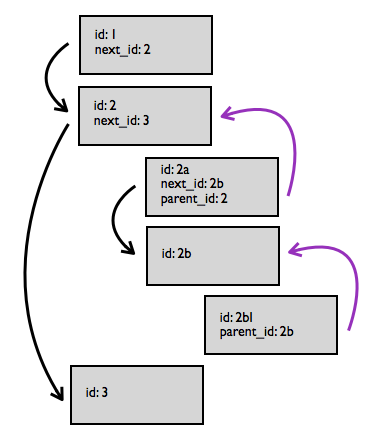
\includegraphics[width=0.6\textwidth]{grafik/pointer} 
  \end{center}
  \caption{The pointer structure}
  \label{fig:pointer}
\end{figure}


Implemented with the pointer structure, the example outline from figure \ref{fig:nestedoutline} will finally look like in listings \ref{lst:theoutline} and \ref{lst:outlineLines}. 

\medskip
\begin{lstlisting}[caption=Chosen implementation of an outline, label={lst:theoutline}]
{
  "_id": "01234567890",
  "kind": "Outline",
  "title": "Shopping list"
}
\end{lstlisting}



\medskip
\begin{lstlisting}[caption=Chosen implementation of three lines, label={lst:outlineLines}]
{
   "_id": "111",
   "kind": "Line",
   "text": "Vegetables",
   "outline_id": "01234567890",
   "next_id": "333",
   "first_note": true
},
{
   "_id": "222",
   "kind": "Line",
   "text": "Carrots",
   "outline_id": "01234567890",
   "parent_id": "111"
},
{
   "_id": "222",
   "kind": "Line",
   "text": "Drinks",
   "outline_id": "01234567890"
}
\end{lstlisting}

This solves the data modelling question. Now all that remains to be determined is how to deal with conflicts that will inevitably occur.

\section{Conflict resolution}
\label{sec:konfliktbehandlung}

As early as 1996, Leslie Knieb developed a distributed database system that allowed distributed storing of data without a locking mechanism \citelit{distributedDBs}. Moreover, the system featured data merging and conflict resolution. Even if the implementation differs from the technology presented here, the requirements are much the same.

Knieb identifies three cases of data synchronisation that do \textit{not} lead to conflicts: changes to a document, creation of a document and deletion of a document \citelit[Chap. 3]{distributedDBs}.

In CouchDB, deletion is regarded as an update to the document. The document is not actually deleted; it simply contains a {\fontfamily{pcr}\selectfont deleted=true} attribute. So \enquote{deletion} will not be regarded as a special case, but rather treated under \enquote{update}. This reduces the number of cases in which conflicts may occur.

The following part discusses the remaining conflicts to be resolved, and how to deal with them. \enquote{Simultaneous} below refers to the time span between two replications of two or more replicas.

\subsection{Simultaneous insertion of a line}
\label{subsec:appendkonfl-arch}

If a new line is created, the line is always conflict-free. However, if several users simultaneously insert a new line in the same place, the previous line (hereinafter simply {\fontfamily{pcr}\selectfont previous}) contains a conflict since its \text{next-pointer} is changed. This conflict is called an \textit{append conflict}. There are two versions of {\fontfamily{pcr}\selectfont previous} that each refer to one of the two newly inserted lines.

An append conflict can be resolved by letting the system store the two new lines into the outline, sorted chronologically and in descending order. The crucial element is the time stamp in the line document. Chronological ordering is suitable for many use cases and it is meaningful to the user. However, since there is no telling whether the clocks on both clients are synchronised, it is primarily a mechanism that offers a single way to resolve this conflict on different clients. It helps avoid situations where a conflict is solved simultaneously but in different ways on two clients, which would lead the system to mistakenly re-recognise a conflict on both clients.

 
\subsection{Simultaneous change of a line}
\label{subsec:writekonfl-arch}

If the text of a document is changed simultaneously by more than one user, conflicts will arise. Even if the new text is the same in both versions, the revision numbers will still differ. This conflict type is called a \textit{write conflict}.

In order to resolve this, instead of the conflicting line, the user is presented with a form that lets her choose from the conflicting versions. She can pick one out and also edit it, i.e. the user can also manually merge both versions.


\subsection{Further conflict types}
\label{subsec:otherconflicts-design}

A special case of change to a document is indentation. For instance, if a user indents a line, this will also become apparent in the documents of other users after the document has been replicated. If, however, a line is indented by one user and outdented by another, it remains to be decided how to present this conflict to the users. A standard solution will depend on how the outliner is actually used.

There are also hybrid types, e.g. if a line is changed and the next is indented. If a write conflict occurs while editing a line and the older version is chosen to resolve the conflict, the line's altered next pointer should be taken into consideration.

Conflicts that happen because of indentation will not be dealt with during the development of the prototype. Also, in order to make things easier, it is assumed that conflicts only occur between two versions. Although not unrealistic in everyday use, there is not enough time to cover this in this thesis. Cases in which an append and a write conflict occur in the same line will however be correctly dealt with.

\subsection{Notification}

The user should be notified when a conflict has occurred after replicating the outline that is currently being edited. This should happen immediately after replication without refreshing the page or interrupting the user in her work. This requirement was set in chapter \enquote{Analysis} (section \ref{subsec:workflow}). Only when the user expressly decides to deal with the conflict, she has to start conflict handling explicitly. The implementation of the notification will be described detailedly in section \ref{subsec:konflikterkennung}.


\section{User interface}

This section will motivate the technologies used in the implementation of the user interface and their architecture.


\subsection{Strategies}

The user interface is to be constructed using simple HTML elements. Complex application frameworks should be omitted; only the jQuery library will be used to make development easier. The use of Adobe Flash was also rejected for the implementation of the outliner. The reason for this is that a DOM tree only uses open web standards in order to better meet expandability and accessibility requirements.

It is easy to build modified or alternative user interfaces for a standards-conform architecture. For example, it would be easy to build a screen reader that reacts to function keys and reads the contents of the lines to the user. The use of CSS makes it easy to change the application's appearance by changing style sheets. The visually impaired can change contrast and font sizes at will. A plug-in that re-formats the outline for print is also conceivable; all it needs to do is traverse the DOM and re-format the individual elements.

Using a Flash or a Sproutcore widget \cite{sproutcore:website} means that the outliner would be a single object, embedded in the site. The contents would thus not be accessible to other technologies. The loading times can also be held at a minimum since the jQuery libraries and the application code are relatively small in size.


\subsection{Site layout}

The application has three views: an overview with a list of all outlines allows the user to change to the single-outline view, which at the same time is the outliner. The third view is the outline edit view where the outline title can be changed or the entire outline deleted.

Newsworthy status information, i.e. notifications, errors or success messages should be shown on the site. They should not be implemented as pop-ups in order not to distract the user from her work. Instead, an HTML element should be shown on the page directly after the event and faded out after a short while by a JavaScript function.

While the application waits for a response from the local database, an animated graphic (a so-called \textit{throbber}) should indicate that the program is working. This provides the user with feedback which eliminates much of the frustration that occurs when the user has to wait a few seconds \citelit{response:miller}.


\subsection{Editor}

The application's core piece is the outliner. It consists of a single page and does not, unlike conventional editors, contain a single text input area. The editor much rather consists of a multitude of text areas. Thus, lines can be sent as individual forms. The text area may be edited at any given time, jumping between them can be done using function keys or the mouse. When a text area loses focus, its contents will be saved immediately. The tree of DOM elements should appear as a single editor window to the user.


\subsection{Interaction}

When the editor is used, it does not interact with the system in the way HTML documents typically do: when the user clicks, the page is requested and loaded from the server. Instead, only some elements on the page will change in response to most interactions. This is done according to the AJAX concept. Both approaches have been more closely examined in \ref{subsec:ajax}, also see figures \ref{fig:classic-interaction-pattern} and \ref{fig:ajax-interaction-pattern}. Following the AJAX method implies that resources are displayed in different states under a single URL. This is contradictory to the REST paradigm presented in section \ref{subsec:rest}, which requires every resource state to have its own address.

The REST concept is breached for a good reason here. If, for instance, a line is added, the corresponding keystroke will change something in the DOM and provoke an HTTP request. This DOM manipulation is, however, minimal and can be performed by a simple JavaScript function. Moreover, the line has to be stored into the database at once. It is crucial that changes to the DOM happen immediately, in order to ensure uninterrupted working. If the user has to wait for a server round-trip in order to see the result of her action, it would take a disproportionally long time.